% Cover letter using letter.cls
\documentclass{article} % Uses 10pt
%\usepackage{helvetica} % uses helvetica postscript font (download helvetica.sty)
%\usepackage{newcent}   % uses new century schoolbook postscript font 
\usepackage[utf8]{inputenc}       % allow Latin1 characters
\usepackage{graphicx}
% the following commands control the margins:
%\topmargin=-1in    % Make letterhead start about 1 inch from top of page 
%\textheight=8.5in    % text height can be bigger for a longer letter
%\oddsidemargin=0pt   % leftmargin is 1 inch
%\textwidth=6.5in     % textwidth of 6.5in leaves 1 inch for right margin
\title{Implementierung eines Temperatur und Luftfeuchtigkeits Sensornetzwerks für den nEDM Experiment Aufbau\\-\\IDP Kurzbeschreibung}
\author{Wenwen Chen, Rainer Schönberger}
\begin{document}
\maketitle
\section*{Das nEDM Experiment}
\subsection*{Überblick}
Nach dem Standardmodell der Teilchenphysik wird derzeit angenommen, dass
Neutronen durch elektroschwache Wechselwirkung ein elektrisches Dipolmoment
in der Größenordnung von etwa $10^{-32}e\cdot cm$ haben. Eine Erweiterung des
Standardmodells wird ein Dipolmoment des Neutrons bereits im Bereich zwischen
$10^{-26}e\cdot cm$ und $10^{-28}e\cdot cm$ vorhergesagt. Derzeit liegt das
Limit für Messungen des Dipolmoments bei ca. $10^{-26}e\cdot cm$\\
Das Neutron EDM Experiment an der TUM versucht deshalb die Messgenauigkeit so
weit zu steigern, damit die oben genannte Theorie entweder belegt oder
widerlegt werden kann.\\
Um dies zu erreichen, werden spinpolarisierte ultrakalte Neutronen (UCN) in
zwei Kammern in einer hochgradig kontrollierten und magnetisch abgeschirmten
Umgebung (siehe Abbildung \ref{fig:exp}) gefüllt. Dort wird dann eine
Spin\-präzessions\-messung nach Ramsey
durchgeführt, mit welcher Informationen über das elektrische Dipolmoment des
Neutrons gewonnen werden.
\begin{figure}[h]
\centering
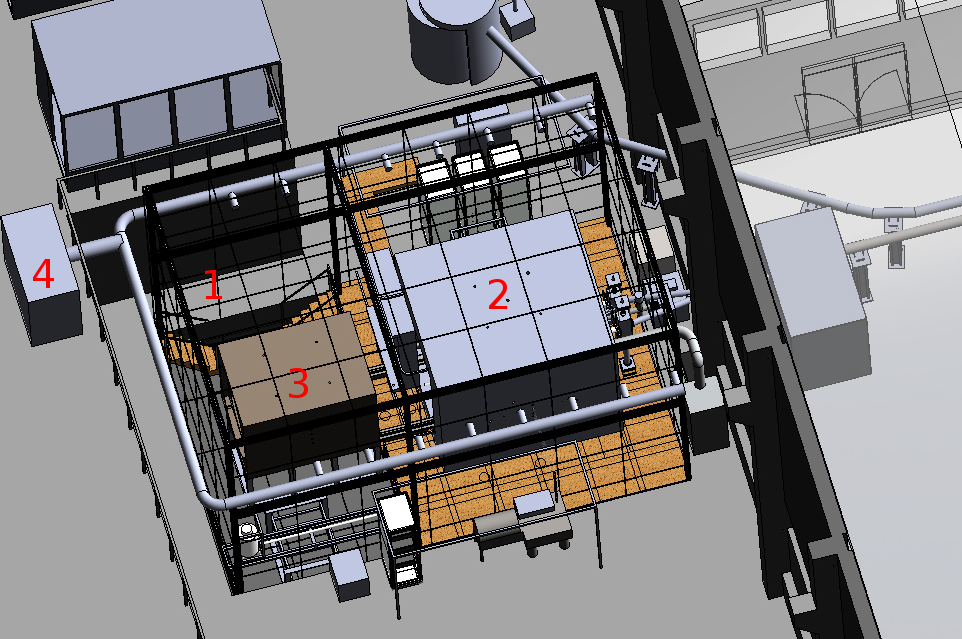
\includegraphics[width=0.7\linewidth]{img/frm3d.png}
\caption{Experiment Umgebung. 1: Spulenkäfig zur magnetischen Feldkompensation,
2: Äußere magnetisches Schild, 3: Inneres magnetisches Schild, 4: Klimaanlage}
\label{fig:exp}
\end{figure}
\subsection*{Notwendigkeit der Umgebungsmessung}
Um sicher zu stellen, dass bei dem Experiment konstante Bedingungen herrschen
ist neben der exakt definierten magnetischen Umgebung auch die 
Umgebungstemperatur, sowie der Luftfeuchtigkeit innerhalb des äußeren
Spulenkäfigs von großer Wichtigkeit. Diese wird von einer Klimaanlage
kontrolliert. Zur Steuerung dieser Anlage muss jedoch die Temperatur an
verschiedenen Positionen im Spulenkäfig gemessen werden.
\section*{Die Vorlesung ``Particle Physics with Neutrons''}
Die Vorlesung behandelt Grundlagen der Neutronenphysik. Sie gibt insbesondere
einen Überblick über die Physik der ultrakalten Neutronen, sowie über einige
experimentelle Methoden im Kontext von Neutronen.\\
Die Vorlesung erlaubt es uns somit, die Hintergründe des nEDM Experiments zu
verstehen, was für die Entwicklung eines Sensornetzwerkes von höchster
Wichtigkeit ist, um die Anforderungen an das Messsystem genau abschätzen zu
können (Genauigkeit, Störungen, Zuverlässigkeit, etc.).
\section*{Unser Projekt}
\subsection*{Überblick}
Das Ziel des Projekts ist Aufbau eines Temperatur- und Luftfeuchtigkeit-
Sensornetzwerks innerhalb des Spulenkäfigs. Die gemessene Temperatur- und 
Luftfeuchtigkeits-Daten sollen im JSON Format per Ethernet geschickt, um 
die Klimaanlagen zu regeln, und in einer 
Datenbank gespeichert werden, zur späteren Korrektur der nEDM Messungen. 
Die gewünschte Datengenauigkeiten sind gelistet in Tabelle \ref{tab:genauigkeit}.
Dazu besteht die folgenden Aufgaben:
\begin{itemize}
\item Recherche nach passender Sensoren 
\item Bewertung der Sensor-Daten
\item Formatierung der Messwert 
\item Datenübertragung per Ethernet
\item Installation des Sensornetzwerks im Experimentaufbau
\item Dokumentieren
\end{itemize}
\begin{table}
  \centering
  \begin{tabular}{|l|c|}
    \hline
    Temperatur-Genauigkeit & 0.1 
    \\ \hline
    Luftfeuchtigkeit-Genauigkeit & 0.1
    \\ \hline
    Daten-Geschwindigkeit & 1s
    \\ \hline
  \end{tabular}
  \caption{Die gewünschte Datengenauigkeiten}
  \label{tab:genauigkeit}
\end{table}
\subsection*{Meilensteine}
Der vorgesehene Zeitplan und Aufgabenaufteilung sind folgendes:
\begin{center}
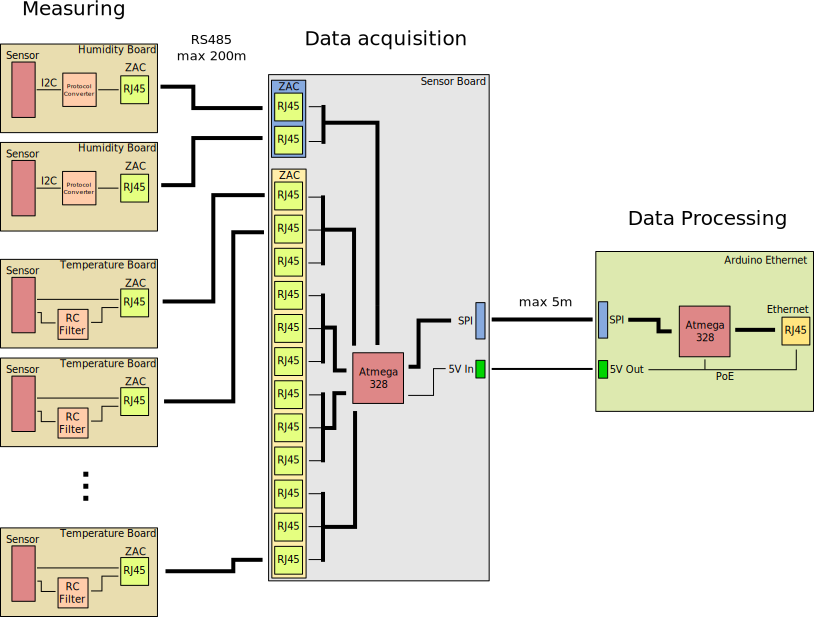
\includegraphics[width=\textwidth]{plan.pdf}
\end{center}
\end{document}
